\clearpage
\section{Phase 2: Polyp Extraction Agent}

Once the navigation problem is solved, we arrive at the real boss fight: Phase 2. This is where the \textbf{SnareNavAgent} takes the stage. The environment here is completely different from Phase 1. Instead of driving through a long tunnel, we spawn the agent right near a pre-positioned polyp inside a ``capture zone.'' Now the agent has to rub its belly and pat its head at the exact same time - it must delicately steer the camera tip \textit{and} precisely manipulate the snare tool simultaneously.


\begin{figure}[H]
\centering
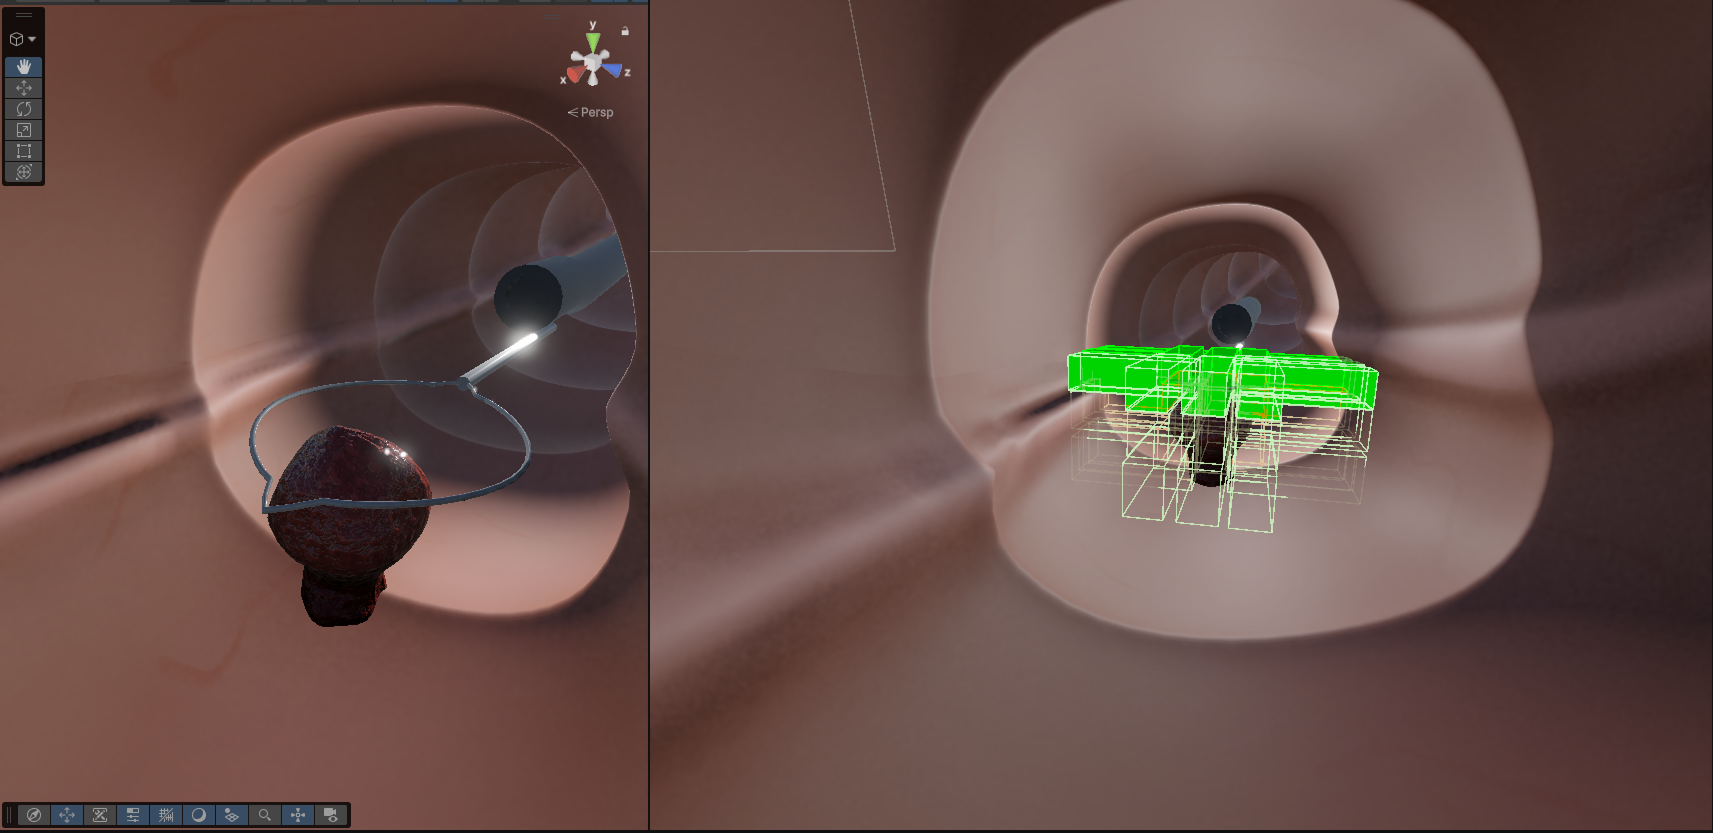
\includegraphics[width=0.8\linewidth]{assets/model-phase2-start.png}
\caption{Phase 2 environment at episode start. Left: the deployed snare near the polyp target. Right: the layered capture zone cubes (green wireframe) used by the \texttt{PolypCaptureZone} reward system.}
\label{fig:phase2_start}
\end{figure}

\subsection{The Multi-Branch Action Space}
To handle this complex dual-control requirement, we set up a \textbf{multi-branch discrete action space}. Instead of a single array of actions, the brain actually outputs \textbf{four separate decisions simultaneously} on every step. Branch 0 controls steering via the familiar \texttt{EndoscopeActionDriver}. Branches 1 through 3 control the snare via the \texttt{SnareSlideController}.

\begin{table}[H]
\centering
\caption{Phase 2: Multi-Branch Action Space}
\label{tab:p2_actions}
\begin{tabular}{|c|l|l|}
\rowcolor{primary}
\textcolor{white}{\textbf{Branch ID}} & \textcolor{white}{\textbf{Control Type}} & \textcolor{white}{\textbf{Discrete Actions Available}} \\
\hline
0 & Steer (WASD) & 0=None, 1=Up, 2=Left, 3=Down, 4=Right \\
\hline
1 & Slide (Extend/Retract) & 0=None, 1=Extend, 2=Retract \\
\hline
2 & Rotate (Twist) & 0=None, 1=Spin Left, 2=Spin Right \\
\hline
3 & Actuate (Open/Close) & 0=None, 1=Open Loop, 2=Close Loop \\
\hline
\end{tabular}
\end{table}

Here is a fun implementation detail: the snare closing animation is not just a simple scale transform! When Branch 3 commands a ``Close Loop'' action, the \texttt{SnareSlideController} actually manipulates a \textbf{SkinnedMeshRenderer blend shape}. It smoothly slides the virtual wire loop into the catheter, clamped strictly to a \textbf{0.7 maximum weight} so it visually matches the physical snare's mechanical limitations. The \texttt{DecisionRequester} runs with a \textbf{period of 5}, meaning the agent makes one decision every 5 physics steps - giving each action time to produce visible consequences before the next decision.

\subsection{The Move-Then-Verify Collision Engine}
One of the trickiest engineering achievements here is how we prevent the snare from magically phasing through the colon wall or the polyp tissue. Standard physics engines struggle terribly with complex, concave, thin-wire collisions.

To solve this, the \texttt{SnareSlideController} implements a very strict \textbf{``move-then-verify''} architectural pattern. Whenever the agent commands a slide, rotate, or blend shape change, the controller:
\begin{enumerate}
\item \textbf{Tentatively applies} the move in memory and instantly bakes the new mesh geometry.
\item Runs an internal \texttt{IsSnareOverlappingBlocker()} function to check for intersections.
\item If \textit{any single vertex} of the snare touches a blocker, it \textbf{immediately reverts} the move and flags the frame as blocked.
\end{enumerate}

But here is where it gets interesting. The virtual simulation cannot natively calculate collisions between two complex concave meshes (like a snare loop and a bumpy colon wall). So we built a \textbf{dual-collision system}:
\begin{itemize}
\item \textbf{High-Fidelity Native Checks:} For the simple spherical polyp colliders, it uses ultra-fast native physics calls (\texttt{OverlapSphereNonAlloc}).
\item \textbf{Vertex-Sampling Fallback:} If it hits the complex colon mesh, it falls back to iterating over the snare's baked vertices, sampling every $N$\textsuperscript{th} vertex and calculating its closest distance to the wall using \texttt{OverlapSphereNonAlloc} on each sample point.
\end{itemize}

There is an interesting temporal quirk: due to the simulation's \texttt{WaitForFixedUpdate} coroutine timing, WASD steering contacts are detected \textbf{one physics step late}, while snare sliding contacts are processed \textbf{instantly in the same step}. The agent actually had to learn to account for this tiny temporal delay!

\subsection{State Space \& The Curiosity Module}
Just like in Phase 1, the Phase 2 agent is entirely \textbf{vision-based}. It uses the exact same $128 \times 128$ CNN visual encoder, the 256-D feature embedding, the 2-layer MLP with Swish activation, and the 128-memory LSTM core. The brain architecture is functionally identical.

However, there is one crucial addition. Capturing a polyp requires extreme precision. The chance of the agent randomly stumbling upon the exact sequence of moves to position the snare, rotate it perfectly, and close it over the polyp is statistically near zero. To help with this, we added an \textbf{Intrinsic Curiosity Module (ICM)} during early training. This module mathematically rewards the agent for encountering \textbf{novel visual states}, encouraging it to poke around the polyp and try weird snare angles instead of just standing still. The ICM runs with a \textbf{strength of 0.02} and its own small neural network (\textbf{64 hidden units}).

The policy head now outputs a \textbf{MultiCategoricalDistribution} with branch sizes $[5, 3, 3, 3]$ (one per action branch). The value network has \textbf{two heads}: one for the extrinsic reward stream and one for the curiosity reward stream.

\subsection{Layered Rewards (The Breadcrumb Trail)}
Because this task is incredibly complex, a simple pass/fail reward just would not work. To fix this, we implemented \textbf{layered spatial rewards} managed by a custom script called \texttt{PolypCaptureZone}.

Think of it like leaving a trail of breadcrumbs for the agent. The zone around the polyp is constructed from \textbf{editor-placed cubes} grouped into \textbf{three concentric layers of 12 cubes each}. A layer becomes active if at least \textbf{6 cubes are occupied} and at least \textbf{one cube is occupied in each quadrant} (left, right, above, behind). This spatial gating ensures the agent genuinely \textit{surrounds} the polyp rather than just poking one side.

\begin{itemize}
    \item \textbf{Layer 1 (Outer Margin):} $+1.5$ reward.
    \item \textbf{Layer 2 (Middle Approach):} $+3.0$ reward.
    \item \textbf{Layer 3 (Inner Core):} $+5.0$ reward.
    \item \textbf{Direct Transition Bonus:} $+2.0$ for consecutive transitions ($1 \rightarrow 2$ or $2 \rightarrow 3$) without backing out.
\end{itemize}

A constant \textbf{step penalty of $-0.001$} pushes the agent to work faster. 

The contact outcomes are extremely strict:
\begin{itemize}
\item \textbf{Small polyp sphere (goal):} Valid \textit{only} in Layer 3. Reward $= 5.0 + 10.0 \times \text{normalizedBlendWeight}$, where $\text{normalizedBlendWeight} = \text{clamp}(\text{blendWeight} / 0.7)$. This means the tighter the snare closes, the bigger the jackpot - up to $+15.0$! Episode terminates successfully.
\item \textbf{Big polyp sphere (penalty):} $-2.0$. Episode continues (the agent gets a chance to correct).
\item \textbf{Colon contact:} $-1.0$ and episode terminates \textit{unless} the agent is in Layer 3 (where we allow some wall grazing during the delicate final approach).
\item \textbf{Close-early penalty:} $-0.01$ if the snare is closed outside Layer 3. This discourages premature snipping.
\end{itemize}


\begin{figure}[H]
\centering
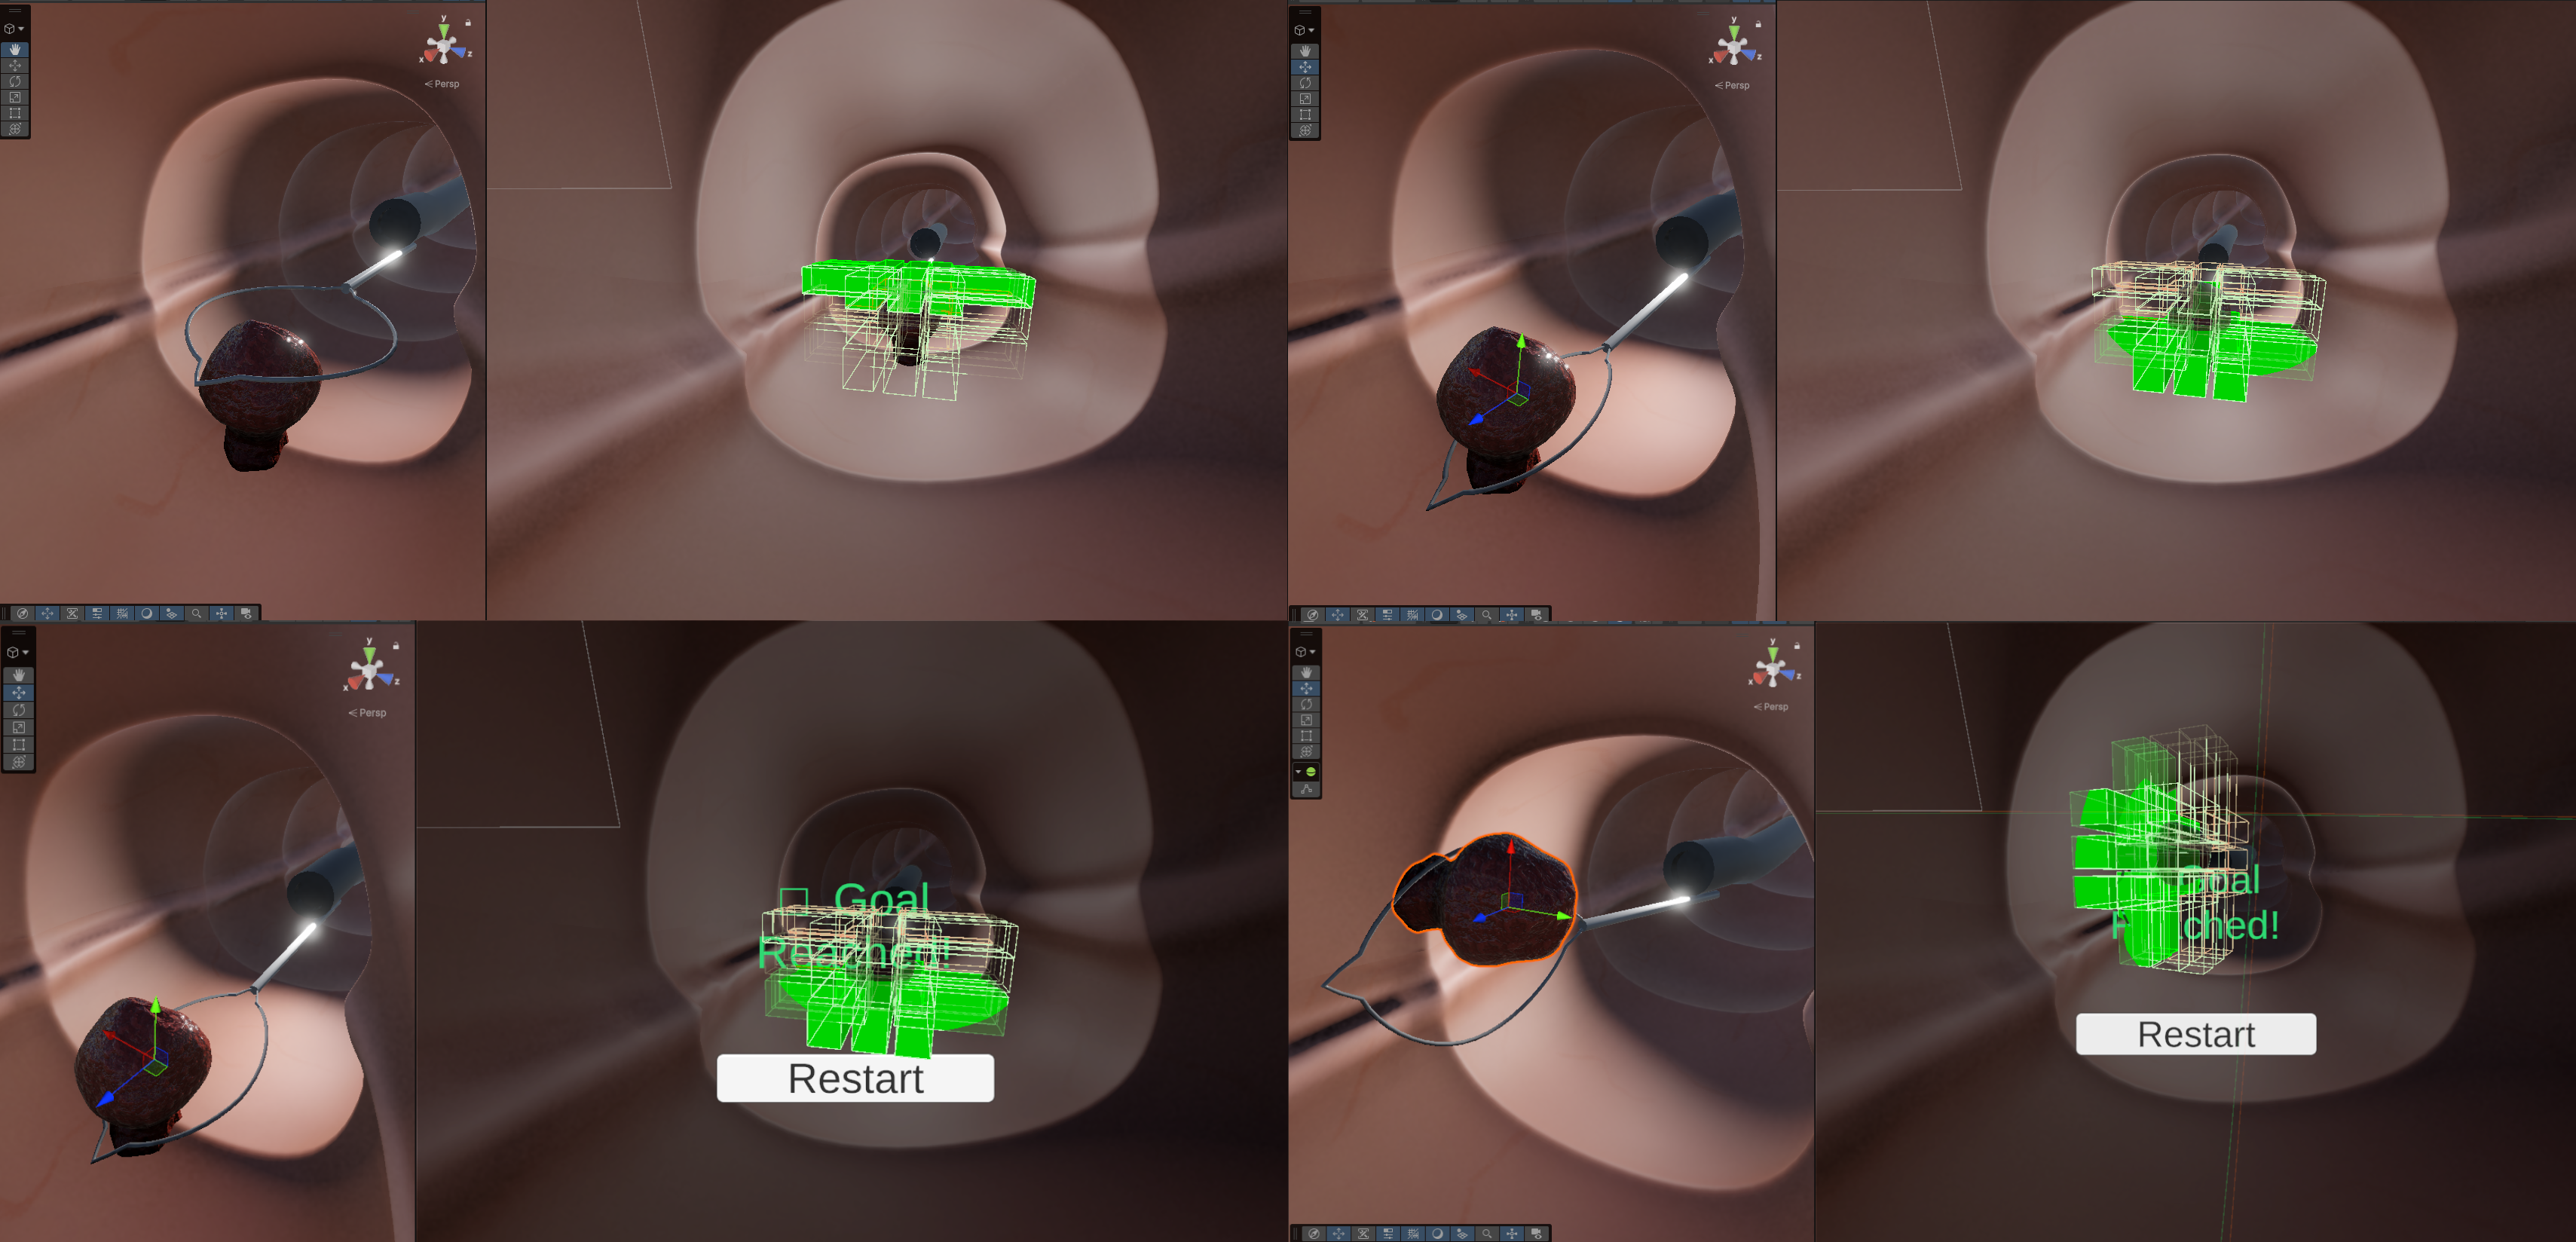
\includegraphics[width=0.8\linewidth]{assets/model-phase2-different-angels.png}
\caption{Multiple capture attempts during Phase 2 training. Each panel pairs the close-up polyp view with the corresponding capture zone state. Bottom panels show successful ``Goal Reached'' episodes.}
\label{fig:phase2_angles}
\end{figure}

\subsection{Episode Reset \& Polyp Randomization}
At the start of each episode, the \texttt{SnareNavAgent} performs a full reset:
\begin{itemize}
\item Resets the rig root to the initial pose and clears push blocked state.
\item Resets snare extension, rotation, and blend weight to zero.
\item Resets the \texttt{PolypCaptureZone} gates and \texttt{PolypContactSensor}.
\item \textbf{Randomly activates} one of the provided tumor GameObjects and updates the contact sensor accordingly.
\end{itemize}

That last point is crucial - by randomizing which polyp is active each episode, we prevent the agent from memorizing a fixed approach trajectory and force it to generalize across different polyp positions and orientations.

\subsection{Training Hyperparameters}
Because Phase 2 requires incredibly delicate, localized movements compared to Phase 1's long-distance driving, we drastically changed the PPO hyperparameters. The batch size drops to \textbf{256} and the buffer to \textbf{2048}, so the agent updates its brain much more frequently based on recent, short interactions with the polyp. We also increased the \textbf{entropy bonus ($\beta$) to 0.01} with a linear schedule to encourage more exploration early on. Training runs for \textbf{1 million steps} with checkpoints saved every 200,000 steps.

\begin{table}[H]
\centering
\caption{Phase 2: PPO Training Hyperparameters}
\label{tab:p2_hyperparameters}
\begin{tabular}{|l|l|}
\rowcolor{primary}
\textcolor{white}{\textbf{Hyperparameter}} & \textcolor{white}{\textbf{Value}} \\
\hline
Algorithm & PPO + Curiosity (ICM) \\
\hline
Batch Size & 256 \\
\hline
Buffer Size & 2048 \\
\hline
Learning Rate & $3 \times 10^{-4}$ (linear schedule) \\
\hline
Entropy Bonus ($\beta$) & $1 \times 10^{-2}$ (linear schedule) \\
\hline
Clip Range ($\epsilon$) & 0.2 (linear schedule) \\
\hline
GAE $\lambda$ & 0.95 \\
\hline
Epochs per Update & 3 \\
\hline
Time Horizon & 128 \\
\hline
Max Training Steps & 1,000,000 \\
\hline
Discount ($\gamma$) & 0.99 \\
\hline
Curiosity Strength & 0.02 \\
\hline
Curiosity Hidden Units & 64 \\
\hline
\end{tabular}
\end{table}

By combining the multi-branch action space, the layered breadcrumb reward system, the curiosity-driven exploration, and the precise move-then-verify collision engine, our Phase 2 agent learns to perform a genuinely complex medical manipulation task entirely from pixel observations. It learns to approach, position, rotate, and close the snare around the polyp stalk - all without a single hard-coded rule or explicit coordinate input!

\subsection{Training Results \& The ``Hacker'' Agent}
Phase 2 proved to be significantly harder to train than Phase 1. To ease the learning curve, we utilized \textbf{transfer learning} across three distinct sub-phases:
\begin{itemize}
\item \textbf{Sub-phase 1:} Best score of \textbf{23.4}, trained for 590,000 steps (took 4.5 hours).
\item \textbf{Sub-phase 2:} Best score of \textbf{26.17}, trained for 610,000 steps (took 2.6 hours).
\item \textbf{Sub-phase 3:} Best score of \textbf{25.73}, trained for 610,000 steps (took 2.1 hours).
\end{itemize}

What made this phase so difficult was that the agent behaved exactly like a \textbf{software hacker}. It constantly probed the environment for glitches, trying to phase through colliders or exploit loopholes in the reward logic to reach the goal without actually performing the intended snaring sequence. Because of this, we had to redesign the collision blocks, the game logic, and the rewards repeatedly. It took an exhausting \textbf{34 attempts} before we finally locked in the right environment!

During this intense training, our most crucial metric wasn't just the average score, but the \textbf{standard deviation}. For example, if the average score was 25 but the standard deviation was 20, it meant the agent was reaching the goal sometimes, but constantly failing while trying weird, alternative glitch methods. Only when the standard deviation dropped down to around \textbf{3} did we know the agent had stopped ``hacking'' and was reliably executing the proper capture maneuver in every single epoch, making it ready for deployment.

\clearpage
